\documentclass[12pt,a4paper]{article}
\usepackage{color}
\usepackage{amsmath}  
\usepackage{amsthm}
\usepackage{amssymb}
\usepackage{amsfonts}
\usepackage{graphicx}  


\begin{document}

\title{Bethe Ansatz Solution of ASEP with Reflecting Boundaries}
\author{Wenwen Huang}
\date{\today}
\maketitle

\section{Single Particle Solution}
\label{sec:single_particle_solution}

To investigate the ASEP model of $N$ particles on $L$ lattice sites with
reflecting boundaries. Let us start with one single particle in such a closed
lattice. The master equation of the particle can be written as
\begin{subequations}
\begin{eqnarray}
    \label{eq:single-particle-a}
    \frac{d}{dt} P(x,t) & = & \alpha P(x-1,t) + \beta P(x+1,t) - (\alpha +
    \beta)P(x,t) \\
    \label{eq:single-particle-b}
    \frac{d}{dt} P(1,t) & = & \beta P(2,t) - \alpha P(1,t) \\
    \label{eq:single-particle-c}
    \frac{d}{dt} P(L,t) & = & \alpha P(L-1,t) - \beta P(L,t)
\end{eqnarray}
\end{subequations}
where $\alpha$ and $\beta$ is hopping rate of particle to left and right,
respectively. $x$ denotes the position of the particle is confined to be the
integer in the range of $1,2,\cdots,L$. Eq.  \eqref{eq:single-particle-b} and
\eqref{eq:single-particle-c} are actually the special cases of master equation
at the boundaries.  By assuming Eq.  \eqref{eq:single-particle-a} is valid for
the whole space, we can rewrite Eq. \eqref{eq:single-particle-b} and
\eqref{eq:single-particle-c} as boundaries condition 
\begin{subequations}
    \label{eq:boundaries-single-particle}
\begin{eqnarray}
    \alpha P(0,t) = \beta P(1,t) \\
    \alpha P(L,t) = \beta P(L+1,t)
\end{eqnarray}
\end{subequations}
The above equations use the technique so called ``ghost coordinate", i.e.
$x=0,L+1$. But physically they are essentially the same as the master equation
\eqref{eq:single-particle-b} and \eqref{eq:single-particle-c}, which means the
flux of particle are balanced in both direction, thus the reflecting boundaries.
The advantage of using Eq. \eqref{eq:boundaries-single-particle} is that it
simplifies the calculation a lot.  

To solve the case of single particle ASEP, we take the ansatz of separation of
variables $P(x,t) = \phi(x)e^{\lambda t}$ and plug into the master equation,
obtaining 
\begin{equation}
    \label{eq:eigen}
    \beta\phi(x+1) -(\alpha+\beta+\lambda)\phi(x) + \alpha\phi(x-1) = 0
\end{equation}
Given that $x$ is an integer number, Eq. \eqref{eq:eigen} is essentially a set
of liner difference equations with the boundaries by substituting the ansatz of
$P_x(t)$ into boundaries of Eq. \eqref{eq:boundaries-single-particle}: 
\begin{subequations}
    \label{eq:boundaries-phi}
\begin{eqnarray}
    \alpha\phi(0) = \beta\phi(1) \\
    \alpha \phi(L) = \beta \phi(L+1)
\end{eqnarray}
\end{subequations}
The standard method to find the solution is again to take an ansatz $\phi(x) =
Az^x$, where $z$ is an arbitrary complex number. We arrive at the characteristic
quadratic equation 
\begin{equation}
    \label{eq:characteristic}
    \beta z^2 - (\alpha + \beta + \lambda ) z + \alpha = 0
\end{equation}
The two roots fulfill $z_1z_2 = \frac{\alpha}{\beta}$. And the solution of
\eqref{eq:eigen} can be written as 
\begin{equation}
    \label{eq:eigen-solution}
    \phi(x) = C_1 z_1^x + C_2 z_2^x
\end{equation}
By applying the boundaries Eq. \eqref{eq:boundaries-phi} to Eq.
\eqref{eq:eigen-solution} we can find all the eigenvalues and corresponding
eigenvectors. The results are summarised as following

\begin{equation}
    \label{eq:single-particle-eigenmodes}
    \begin{aligned}
        \lambda_s & = 0; 
        ~\phi_s(x) = const. \left(\frac{\alpha}{\beta}\right)^{x}; \\
        \lambda_k & = -(\alpha+\beta) +
        2\sqrt{\alpha\beta}\cos(\frac{k\pi}{L}); 
        ~k=1,2,\dots, L-1 \\
        \phi_k(x) & = const. \left(\frac{\alpha}{\beta}\right)^{\frac{x}{2}}
            \left[\sin\left(\frac{k\pi}{L}x\right) -
                \sqrt{\frac{\beta}{\alpha}}\sin\left(\frac{k\pi}{L}(x-1)\right)\right].
    \end{aligned}
\end{equation}
% \begin{subequations}
%     \label{eq:single-particle-eigenvalues}
%     \begin{eqnarray}
%         \lambda_k & = &
%         \begin{cases}
%             -(\alpha+\beta) + 2\sqrt{\alpha\beta}\cos(\frac{k\pi}{L});
%             & k=1,2,\dots, L-1 \\
%             0; & k=L
%         \end{cases}
%     \end{eqnarray}
%     \label{eq:single-particle-eigenvectors}
%     \begin{eqnarray}
%         \phi_k(x) & = & 
%         \begin{cases}
%             const. \left(\frac{\alpha}{\beta}\right)^{\frac{x}{2}}
%             \left[\sin\left(\frac{k\pi}{L}x\right) -
%                 \sqrt{\frac{\beta}{\alpha}}\sin\left(\frac{k\pi}{L}(x-1)\right)\right];
%             & k = 1,2, \dots, L-1 \\
%             const. \left(\frac{\alpha}{\beta}\right)^{x}; & k=L
%         \end{cases}
%     \end{eqnarray}
% \end{subequations}
The eigenvalue $\lambda_s = 0$ and corresponding eigenvector represent the
stationary mode $\phi_s(x)$. Define a scalar product between any two functions
by \begin{equation} \label{eq:scalarPoduct} (\phi, \psi) =
    \int\frac{\phi(x)\psi(x)}{\phi_{s}(x)}dx 
\end{equation}
Notice that definition Eq. \eqref{eq:scalarPoduct} makes $\phi_s(x)$ identical
to the stationary distribution $P^e(x)$.
By properly choose the constant and when $L\rightarrow\infty$,
one can check the orthogonality and completeness of the eigenfunctions.
\begin{eqnarray}
    \label{eq:orthogonality}
    \sum_{x=1}^L \phi_k(x)\phi_l(x) & = & \delta_{k,l} \\
    \label{eq:completeness}
    \sum_{k=1}^L \phi_k(x)\phi_k(y) & = & \delta_{x,y} 
\end{eqnarray}
So for arbitrary initial distribution of $P(x, 0)$, we can always decompose it as 
\begin{equation}
    \label{eq:decompose-intial-single}
    P(x,0) = \sum_k{c_k \phi_k(x)}
\end{equation}
where $c_k$ can be calculated by 
\begin{equation}
    \label{eq:coeff-k}
    c_k = \sum_x{\phi_k(x) P(x,0)}
\end{equation}
Finally, the solution of single particle on reflecting lattice can be written as
\begin{equation}
    \label{eq:solution-single}
    P(x,t) = \sum_k{\phi_k(x)e^{\lambda_k
            t}}\sum_{x^\prime}{\phi_k(x^\prime)P(x^\prime,0)}
\end{equation}
For the special case that $P(x,0) = \delta_{x,y}$, solution
\eqref{eq:solution-single} can be simplified to
\begin{equation}
    \label{eq:solution-single-simplified}
    P(x,t) = \sum_k{\phi_k(x)\phi_k(y)e^{\lambda_k t}}
\end{equation}

With the complete solution of single particle, we can go further to systems of
more than one particle. The idea is that the single particle solution works as
building blocks for the $N$ particle solutions. To start with that, we first
illustrate the case $N=2$ and the position of particles are denotes by $x_1,
x_2$ with constraint $x_1<x_2$.

\section{Solution of Two Particles}
\label{sec:solution_of_two_particles}
Firstly, we shall write down the master equation, which looks as following
\begin{equation}
    \begin{aligned}
    \label{eq:masterEqTwo}
    \frac{d P(x_1, x_2; t)}{dt} = & \alpha P(x_1-1,x_2;t) + \beta P(x_1+1,x_2;t) \\ 
    & + \alpha P(x_1, x_2-1; t) + \beta P(x_1, x_2+1; t)  \\ 
    & - 2(\alpha+\beta)P(x_1, x_2; t)
    \end{aligned}
\end{equation}
And the reflecting boundaries write as
\begin{subequations}
    \label{eq:boundaries-two-particles}
    \begin{eqnarray}
        \alpha P(0,x_2; t) = \beta P(1, x_2, t) \\
        \alpha P(x_1, L;t) = \beta P(x_1, L+1;t)
    \end{eqnarray}
\end{subequations}
For the case of more than one particle, we need to take into account the
exclusion effect, i.e., one site can be occupied by at most one particle.
This can be also written as a boundary condition as 
\begin{equation}
    \label{eq:exclusionCondition}
    \alpha P(x, x; t) + \beta P(x+1, x+1; t) = (\alpha + \beta) P(x, x+1; t)
\end{equation}
Notice that the exclusive condition must hold for any $x$. The notation of $P(x,
x; t)$ may looks a little bit weird, but keep in mind that it is a boundary condition
that denotes the limiting situation $x_1=x_2$.

The idea to construct the $N$ particle solution is inspired by the standard
Coordinate Bethe Ansatz (CBA). However, instead of using the plain plane wave
function as building blocks, we use the eigenfunctions of single particle
solution. To show that, we need to again do the eigenfunction expansion of the
solution, which can be written as 
\begin{equation}
    \label{eq:solutionTwo}
    P(x_1, x_2, t) = \sum_{k} \Psi_{k}(x_1, x_2) e^{\lambda_k t}
\end{equation}
The key point here is the construction of $\Psi(x_1, x_2)$. We take the Ansatz
that the general form of $\Psi(x_1, x_2)$ can be written as
\begin{equation}
    \label{eq:solutionTwoEigenFunc}
    \Psi(x_1, x_2) = A_{12}\psi_1(x_1)\psi_2(x_2) +
    A_{21}\psi_2(x_1)\psi_1(x_2)
\end{equation}
Plug in to the master equation Eq. \eqref{eq:masterEqTwo} we arrive at
\begin{subequations}
    \label{eq:subMasterEqTwo}
    \begin{eqnarray}
        \alpha\psi_1(x-1) + \beta\psi_1(x+1) - 
        (\alpha+\beta+\lambda)\psi_1(x) = 0 \\
        \alpha\psi_2(x-1) + \beta\psi_2(x+1) - 
        (\alpha+\beta+\lambda)\psi_2(x) = 0
    \end{eqnarray}
\end{subequations}
One can readily find $\psi_1(x)$ and $\psi_2(x)$ should be the eigenfunction of
single particle master equation, respectively. So we use the solution of
section \ref{sec:single_particle_solution} with unfixed coefficients as trial
function and keep in mind the exclusive condition should be fulfilled. In the
following text, we will discuss several different cases separately.

\subsection{Stationary Solution}
\label{sub:stationary_soution}
Let us first check the case $\psi_1(x) = \psi_2(x) = \phi_s(x)$. Namely
\begin{equation}
    \label{eq:stationaryTwo}
    P^e(x_1, x_2) = \Psi(x_1, x_2) = A \left(\frac{\alpha}{\beta}\right)^{x_1+x_2}
\end{equation}
This will lead to the stationary solution as one would expected. First, we can
easily obtain from Eq. \eqref{eq:subMasterEqTwo} and Eq.
\eqref{eq:solutionTwoEigenFunc} that the corresponding eigenvalue $\lambda_k=0$.
And then one can check easily the exclusive condition Eq.
\eqref{eq:exclusionCondition} is fulfilled. 

The prefactor $A$ can be fixed by normalization. However, it is not a trivial
work because of the constraint $x_1 < x_2$. We will discuss in detail in
general case of $N$ later. 

\subsection{Non-stationary Modes}
\label{sub:non_stationary_modes}
We now check the case $\psi_1(x) = \phi_s(x)$, $\psi_2 = \phi_k(x),
k=1,2,\cdots,L-1$. The exchange of $\psi_1$ to $\psi_2$ makes the identical
results. So we can write the solution as 
\begin{equation}
    \label{eq:nonstationaryModesTwo}
    \Psi(x_1, x_2) = A_{12} \left(\frac{\alpha}{\beta}\right)^{x_1}\phi_k(x_2) 
    + A_{21} \left(\frac{\alpha}{\beta}\right)^{x_2}\phi_k(x_1) 
\end{equation}
We first insert the solution to the master equation Eq. \eqref{eq:masterEqTwo},
obtaining the corresponding eigenvalue $\lambda_k = -(\alpha+\beta) + 
2\sqrt{\alpha\beta}\cos(\frac{k\pi}{L})$.

We now check the exclusive condition Eq. \eqref{eq:exclusionCondition}. Simply
substitute Eq.  \eqref{eq:nonstationaryModesTwo} into the condition. In order to
fulfill the exclusive condition, we find that $A_{12} / A_{21} =  \alpha /
\beta$.

Finally, insert Eq. \eqref{eq:boundaries-single-particle} in to
Eq. \eqref{eq:boundaries-two-particles}, we can check that $\phi_k(x)$ must
choose to be exactly the single particle eigenfunction to fulfill the
reflecting boundaries.

Here we summarize the non-stationary eigenvalues and corresponding
eigenfunctions for the two particles ASEP. 
\begin{subequations}
    \label{eq:eigenTwo}
    \begin{eqnarray}
        \label{eq:eigenvaluesTwo}
        \lambda_k & = &
        -(\alpha+\beta) + 2\sqrt{\alpha\beta}\cos(\frac{k\pi}{L});
        ~k=1,2,\dots, L-1  \\
        \label{eq:eigenvectorsTwo}
        \Psi(x_1, x_2) & = & A\left[ \frac{\alpha}{\beta} \left(\frac{\alpha}{\beta}
            \right)^{x_1}\phi_k(x_2)+\left(\frac{\alpha}{\beta}\right)^{x_2}
            \phi_k(x_1) \right]
    \end{eqnarray}
\end{subequations}

Finally, we want remark here, the eigenfunctions listed in Eq.
\eqref{eq:eigenTwo} are not the complete set of non-stationary eigenfunctions,
we will leave the discussion of this issue to next section. 

\section{General Solution of $N$ particles ASEP}
\label{sec:general_solution_of_n_particles_asep}

As before, we first write down the master equation of a $N$ particles system.
\begin{equation}
    \begin{aligned}
        \label{eq:masterEqN}
        \frac{d P(x_1, \cdots, x_N; t)}{dt} = & \sum_{j=1}^N \left[\alpha
            P(\cdots,x_j-1,\cdots;t) + \beta P(\cdots, x_j+1, \cdots;t)\right. \\ 
        & \left.- (\alpha+\beta)P(\cdots, x_j, \cdots; t)\right]
    \end{aligned}
\end{equation}

Similarly, the reflecting boundaries write as
\begin{subequations}
    \label{eq:boundaries-N-particles}
    \begin{eqnarray}
        \alpha P(0,x_2,\cdots,x_N; t) = \beta P(1, x_2,\cdots, x_N; t) \\
        \alpha P(x_1,\cdots, x_{N-1}, L;t) = \beta P(x_1,\cdots, x_{N-1}, L+1;t)
    \end{eqnarray}
\end{subequations}
The exclusive condition for $N$ particles case is more tricky. In principle,
one has to consider to case of three body collision and four body collision and
so on. Luckily, in the simple model of ASEP, one can prove that these more than
two body exclusive conditions are not new but just linear recombination of two
body exclusive condition. So we can write the exclusive condition of a $N$
particles system as 
\begin{equation}
    \label{eq:exclusionConditionN}
    \alpha P(\cdots,x, x,\cdots; t) + \beta P(\cdots, x+1, x+1, \cdots; t) 
    = (\alpha + \beta) P(\cdots, x, x+1, \cdots; t)
\end{equation}

The procedure of searching solution in section
\ref{sec:solution_of_two_particles} can be generalize to $N$ particles case in a
straight forward manner. Let us again start with the stationary solution. 

\subsection{Stationary Solution}
\label{sub:stationary_solution}

Intuitively, we construct the $N$ particles stationary solution as
\begin{equation}
    \label{eq:stationaryN}
    P^e(x_1, x_2, \cdots, x_N) = \Psi(x_1, x_2, \cdots, x_N) =  A
    \prod_{j=1}^N\left(\frac{\alpha}{\beta}\right)^{x_j}
\end{equation}

One can plug in the master equation check that the corresponding eigenvalue
$\lambda= 0$, and also verify the exclusive condition as well as the reflecting
boundaries are fulfilled by insert the solution in to Eq.
\eqref{eq:exclusionConditionN} and Eq. \eqref{eq:boundaries-N-particles}
separately.

We now try to fix the parameter $A$ by normalization. Let us denote
$q:=\frac{\alpha}{\beta}$, then we can write $A$ as following
\begin{equation}
    \label{eq:stationaryPrefactor}
    A^{-1} = \sum_{\Omega} q^{\sum_j{x_j}} = 
    \sum_{x_1 < x_2 < \cdots < x_N} q^{\sum_j{x_j}}
\end{equation}
Let us do a variable change so that 
\begin{eqnarray*}
    \sum_j{x_j} &=& E_0 + E \\
    E_0 &=& 1 + 2 + \cdots + N = \frac{N(N+1)}{2}
\end{eqnarray*}
We can derive that $E$ is a integer in the range of $0, 1, \cdots, N(L-N)$. So
Eq. \eqref{eq:stationaryPrefactor} can be rewrite as 
\begin{equation}
    \label{eq:prefactorRewrite}
    A^{-1} = q^{E_0}\sum_{E=0}^{N(L-N)}g(E)q^E
\end{equation}
where $g(E)$ is the number of partitions of positive integer $E$ to $N$ parts
with each of size at most $L-N$. From the number partition theory, we identify
\begin{equation}
    \label{eq:degeneratcy}
    \sum_{E=0}^{N(L-N)}g(E)q^E = \binom{L}{N}_q =
    \frac{[L]_q!}{[L-N]_q![N]_q!}
\end{equation}
where $[N]_q = 1 + q + q^2 + \cdots + q^{N-1}$ is called a $q$ number, and Eq.
\eqref{eq:degeneratcy} is called the $q$ binomial coefficient\cite{}.
So we finally arrive at 
\begin{equation}
    \label{eq:stationarySolutionN}
    P^e(x_1, x_2, \cdots, x_N) = q^{-\frac{N(N+1)}{2}}
    \binom{L}{N}_q^{-1}\prod_{j=1}^N{q^{x_j}}
\end{equation}

In \cite{}, G. M. Sch\"{u}tz use a quantum group formalism obtained the same
result with a different notation. We emphasize here that our method is much more
easily to understand and no prerequisite knowledge of quantum mechanics and
group theory is needed.

With the equilibrium $N$ particle distribution, we can readily calculate the
equilibrium distribution of any tagged particle. Denote he distribution of the
$k$th particle $p_k(x)$, we have
\begin{equation}
    \begin{aligned}
        \label{eq:pdfTaggedParticle}
        p_k(x) = & \sum_{0<x_1<\cdots<x_{k-1}\le x-1}P^e(x_1, x_2, \cdots, x_N)
        \sum_{x<x_{k+1}<\cdots<x_{N}\le L}P^e(x_1, x_2, \cdots, x_N) \\
        = & \left. q^{(N+1-k)(x-k)} \binom{x-1}{k-1}_q\binom{L-x}{N-k}_q 
            \middle/  \binom{L}{N}_q \right.
    \end{aligned}
\end{equation}
Finally, the equilibrium density profile can be obtain by summing up $p_k(x)$
\begin{equation}
    \label{eq:densityProfile}
    \rho(x) = \sum_{k=1}^N p_k(x) 
\end{equation}


\subsection{Non-stationary Modes}
\label{sub:non_stationary_modes}

Inspired by the two particle calculation, we start to searching for $N$
particle non-stationary eigenfunctions by taking the following Ansatz
\begin{equation}
    \label{eq:nonstationaryModesN}
    \begin{aligned}
        % \Psi(x_1, x_2, \cdots, x_N) = & A_{1}\phi_k(x_1)\prod_{j\neq
        %     1}\left(\frac{\alpha}{\beta}\right)^{x_j} + \cdots \\ 
        % & + A_{k}\phi_k(x_k)\prod_{j\neq k} 
        % \left(\frac{\alpha}{\beta}\right)^{x_j}+\cdots 
        % \\ & + A_{N}\phi_k(x_N)\prod_{j\neq
        % N}\left(\frac{\alpha}{\beta}\right)^{x_j} 
        \Psi(x_1, x_2, \cdots, x_N) = \sum_{k=1}^N
         A_{k}\phi_k(x_k)\prod_{j\neq k} 
         \left(\frac{\alpha}{\beta}\right)^{x_j}
    \end{aligned}
\end{equation}

We again insert the solution to the master equation Eq. \eqref{eq:masterEqN},
obtaining the corresponding eigenvalue $\lambda_k = -(\alpha+\beta) + 
2\sqrt{\alpha\beta}\cos(\frac{k\pi}{L})$.

By substitute Eq. \eqref{eq:nonstationaryModesN} into the exclusive condition
Eq. \eqref{eq:exclusionConditionN}, we get $A_{k+1} / A_{k} =  \alpha /
\beta$.

Finally, the reflecting boundary condition can be checked by choosing
$\phi_k(x)$ be exactly the single particle eigenfunctions.

The results are summarized as following:  
\begin{subequations}
    \label{eq:eigenN}
    \begin{eqnarray}
        \label{eq:eigenvaluesN}
        \lambda_k  = 
        -(\alpha+\beta) + 2\sqrt{\alpha\beta}\cos(\frac{k\pi}{L});
        ~k=1,2,\dots, L-1  \\
        \label{eq:eigenvectorsN}
        \Psi(x_1, x_2, \cdots, x_N)  =  A \sum_{k=1}^N
        \left(\frac{\alpha}{\beta}\right)^{k-1} \phi_k(x_k)\prod_{j\neq k} 
         \left(\frac{\alpha}{\beta}\right)^{x_j}
    \end{eqnarray}
\end{subequations}


\subsection{Completeness of Eigenfunctions}
\label{sub:completeness_of_eigenfunctions}

Although we found some non-stationary eigenmodes listed in Eq.
\eqref{eq:eigenN}. We have to say, this is not a complete set of all
eigenmodes. This can be checked by counting the number of independent
eigenfunctions. For a discrete system like $N$ particles on $L$ lattice sites,
there dimension of the configuration space is $\binom{L}{N}$. So the transition
matrix should has $\binom{L}{N}$ independent eigenvectors. However, we only
found $N$ instead of $\binom{L}{N}$.

The possible remaining eigenfunctions, as one may expect intuitively, can be
constructed by combination of non-stationary single particle eigenfunctions. 
We can write them as following
\begin{equation}
    \label{eq:possibleEigenModes}
    \Psi(x_1, x_2, \cdots, x_N) = \sum_{\sigma\in S_N}
    A_{\sigma(k)}\prod_{k} \phi_k(x_{\sigma(k)})
\end{equation}
The expanded example of simple two particles case reads
\begin{equation}
    \label{eq:possibleEigenModesTwo}
    \Psi(x_1, x_2, \cdots, x_N) = A_{12}\phi_k(x_1)\phi_l(x_2)
    + A_{21}\phi_k(x_2)\phi_l(x_1)
\end{equation}

Because $\phi_k(x)$ is exactly the eigenfunction of a single particle on the
lattice box $[1,L]$, the reflecting boundaries Eq.
\eqref{eq:boundaries-N-particles} can be checked being fulfilled easily. 

So we only need to tale care of the exclusive condition Eq.
\eqref{eq:exclusionConditionN}. We can simply plug in the general form of
$\phi_k(x)$ with unfixed parameters
\begin{equation}
    \label{eq:generalPhik}
    \phi_k(x) = A\left(z^x + B q^x z^{-x}\right)
\end{equation}

We found the exclusive condition will be satisfied if we choose $A_{\sigma(k)}
/ A_{\sigma(l)} = 1,~z_k \neq z_l$ or $z_k = z_l = \pm \sqrt{\alpha/\beta}$.
The later case can be eliminated because the reflecting boundaries Eq.
\eqref{eq:boundaries-N-particles} will not be satisfied if we resubstitute into
the equations.

{\color{red} It looks like all good in the calculations. But the problem is if we
    assume this is true, then we should expect the corresponding eigenvalue for
    the $N$ particles system combined by single particle eigenvalues such like
    $\lambda = \lambda_k + \lambda_l;~k,l = 1, 2, \cdots, L-1;~k\neq l$.
    However, there are at least two contradictions. The First one is we don't
    see this sort of eigenvalues if we diagonalize the transition matrix
    numerically, instead we see something else. The second one is the total
    number of eigenfunctions can not sum up to $\binom{L}{N}$. So either we have
    missed something here or somewhere is wrong in my calculation, which I
    checked for many times. }

\section{Relaxation Time}
\label{sec:relaxation_time}

Although we can not get the complete set of eigenvalues and eigenfunctions
analytically, we can still postulate the largest non-zero value is contained in
the set we already found. The largest non-zero eigenvalue we found is 
\begin{equation}
    \label{eq:largestEigenvalue}
    \lambda_1 = -(\alpha+\beta) +
    2\sqrt{\alpha\beta}\cos(\frac{\pi}{L})
\end{equation}
If $L\ll 1$, we can expand the cos term, obtain 
\begin{equation}
    \label{eq:largestEigenvalueExpanded}
    \lambda_1 = -(\sqrt{\beta}-\sqrt{\alpha})^2 +
    \frac{\sqrt{\alpha\beta}\pi^2}{L^2}
\end{equation}
And the relaxation time can be calculated as 
\begin{equation}
    \label{eq:relaxationTime}
    \tau = -\frac{1}{\lambda_1}
\end{equation}

There are several information we can read form Eq.
\eqref{eq:largestEigenvalueExpanded} and \eqref{eq:relaxationTime}. Firstly, we
can see the scaling $\tau \approx L^2$, which means the dynamical exponent of
the system is $2$. Secondly, as we can see from Eq.
\eqref{eq:largestEigenvalueExpanded}, the bigger difference between $\alpha$
and $\beta$, the smaller relaxation time we will get. This is also consistent
as one would expect. If we map back to the polymer model, the result here can
be compared with the prediction of Rouse theory. Unlike the prediction
from Rouse theory that relaxation time does not depend on external force, we
have here that stronger external force decreases the relaxation time. This
point highlight the fundamental difference between the infinite extensible bead
spring model and the rigid bead rod model which is of course finite extensible. 

We want to remark here that it would be a hard mathematical problem to prove
Eq. \eqref{eq:largestEigenvalue} leads to the correct relaxation time of the
system. Even if we can found all the eigenfunctions, the proof might become a
problem of comparing the roots of a polynomial equation to $\lambda_1$ listed
here. Because the remaining eigenvalues are related to polynomial equations as
hinted by the numerical diagonalize of transition matrix. However, we can still
show the numerical evidence of the postulate above, e.g. Fig.
\ref{fig:eigenvalues} shows all the eigenvalues of a system with $L=10$
lattice sites with the number of particles from $1$ to $9$. The transition
matrix was diagonalize numerically here. The difficult to calculate larger
lattice size $L$ lies on that the dimension grow as $\binom{L}{N}$, and if we
take $N=L/2$, the dimension of the matrix will became a extremely large number
very soon. 

\begin{figure}[htpb]
    \centering
    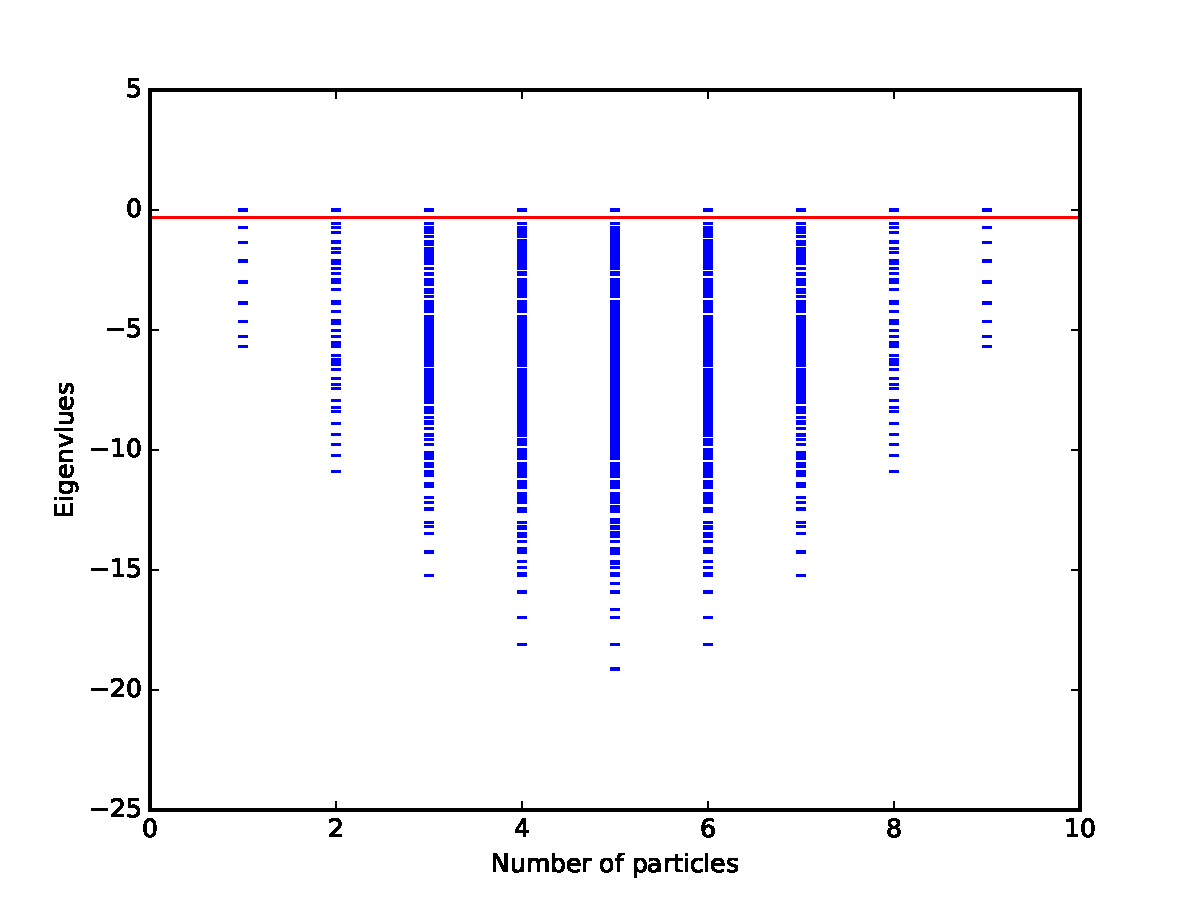
\includegraphics[width=0.8\linewidth]{eigenvalues}
    \caption{Eigenvalues calculated by numerically diagonalize the transition
        matrix.}
    \label{fig:eigenvalues}
\end{figure}

Actually, there are more information hinted by Fig. \ref{fig:eigenvalues}.
One can see that all eigenvalues of case $N=1$ are contained in the set of
eigenvalues $N=2$, and all eigenvalues of case $N=2$ are contained in the set
of $N=3$ and so on until reach the largest set $N=L/2$. This means the
characteristic polynomial of $N=k+1$ always contains the factor of the
characteristic polynomial $N=k$. This is verified by the calculation started
from the simplest case $N=2$ and $L=4$.

\section{Summary}
\label{sec:summeary}
We use the modified Bethe Ansatz methods solve the ASEP model with reflecting
boundaries.  Although the complete set of eigenvalues and eigenfunctions were
not found, the stationary distribution was solved exactly and the one
correspond to the relaxation time of the system was postulated. Numerical
evidence is provided for later statement.


% \bibliography{report}
\bibliographystyle{plain} 

\end{document}
